
\chapter{Projekt i implementacja algorytmu generującego plan lekcji}

\section{Wstęp}
Problem ułożenia najlepszego planu zajęć jest problemem NP-zupełnym. W projekcie zostało zaimplementowane podejście ewolucyjne. Na~rysunku~\ref{rys:time_table_dia} została zobrazowana struktura generowanego planu zajęć.

\begin{figure}[h]
\centering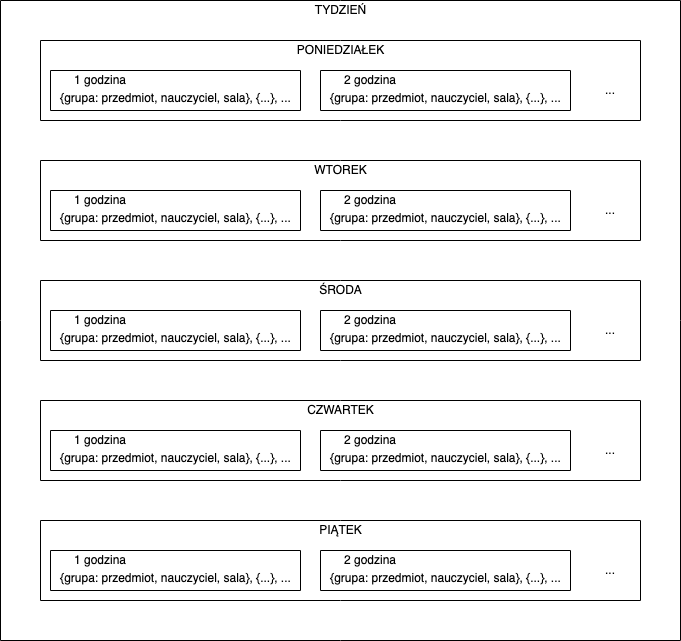
\includegraphics[width=14cm]{figures/time_table_dia}
\caption{Struktura planu zajęć}\label{rys:time_table_dia}
\end{figure}


Zagadnienie implementacji algorytmu można podzielić na cztery główne części: 
\begin{itemize}
	\item przygotowanie danych wejściowych,
	\item ułożenie planu zajęć,
	\item ocena planu zajęć,
	\item ewolucja planu zajęć.
\end{itemize}

\section{Przyjęte założenia}
Przyjęte zostało, że: 
\begin{itemize}
	\item grupa jest najmniejszą, niepodzielną jednostką szkolną (oznacza to, że w jednej grupie nie mogą znajdować się żadne inne podgrupy, dla których konieczne byłoby odzielne ułożenie planu),
	\item sale nie mają określonego limitu uczniów,
	\item grupy nie mają określonej liczby uczniów.
\end{itemize} 


\section{Narzędzia}
Algorytm został zaprogramowany w języku \textit{Python}. Pozwoliło to na szybkie wdrażanie zmian do kodu źródłowego algorytmu. Dużą zaletą wspomnianego języka jest jego prostota i czytelność, co w przypadku tak złożonego zagadnienia, jak algorytm generujący plany zajęć jest niezwykłe ważne. \textit{Python} automatycznie zarządza pamięcią, Programista nie musi zwracać uwagi na zagadnienia związanie np. z uwalnianiem pamięci po nieużywanych zasobach, co powoduje, że \textit{Python} jest językiem bezpieczniejszym niż np. \textit{C++}.

\section{Zastosowanie algorytmu ewolucyjnego}
Algorytm wykorzystuje podejście ewolucyjne, z wykluczeniem mechanizmu krzyżowania. Z połączenia dwóch różnych planów zajęć trudne jest utworzenie trzeciego. Dlatego też, algorytm w celu ewolucji planów zajęć, korzysta wyłącznie z mechanizmu mutacji. Oznacza to, że każdy nowowygenerowany plan zajęć posiada wyłącznie jednego rodzica.

\section{Przygotowanie danych wejściowych}
    
    Przygotowanie danych wejściowych jest kluczowe w działaniu algorytmu. Na podstawie danych otrzymanych od back-end, zostaje ułożona lista czteroelementowych krotek, gdzie pierwszym elementem jest nazwa klasy, drugim elementem jest nazwa przedmiotu, trzecim elementem jest nazwa nauczyciela, a czwartym elementem jest nazwa sali. Wartość elementu sali jest na początku wartością pustą null, a wartość elementu nauczyciela, jest wartością pustą null, wtedy i tylko wtedy kiedy nie został wskazany nauczyciel dla konkretnej klasy. W takiej liście znajdują się wszystkie jednostki lekcyjne występujące w całej szkole. Przykładowo jeżeli pewna klasa IIC ma mieć 5 matematyk w tygodniu z nauczycielem Jan Kowalski, to do listy dostanie dodane pięć krotek postaci (IIC, matematyka, Jan Kowalski, null). Struktura wspomnianej listy znajduje się na ~rysunku~\ref{rys:krotki}.


\begin{figure}[h]
\begin{tabular}{llll}
NAZWA GRUPY & NAZWA PRZEDMIOTU & NAZWA NAUCZYCIELA & NAZWA SALI \\
IIC         & matematyka       & Jan Kowalski      & null       \\
IIC         & matematyka       & Jan Kowalski      & null       \\
IIC         & matematyka       & Jan Kowalski      & null       \\
IIC         & język polski     & Andrzej Nowak     & null       \\
IIC         & język polski     & Andrzej Nowak     & null       \\
IA          & język polski     & null              & null      
\end{tabular}
\caption{Struktura listy krotek} \label{rys:krotki}
\end{figure}

\section{Ułożenie poprawnych planów zajęć}

    Głównym założeniem układania planu zajęć jest to, że na podstawie tej samej listy krotek, zawsze zostanie wygenerowany konkretny plan zajęć. 
Układanie planu zajęć przebiega następująco:
\begin{enumerate}
	\item z listy krotek zostaje zabrana pierwsza z brzegu krotka,
	\item wybrana krotka zostaje przydzielona do pierwszej możliwej konkretnej godziny w 		\item konkretnym dniu (czyli do takiej jednostki godzinowej, wtórej są spełnione 			\item wprowadzone przez użytkownika założenia oraz jest wolna sala),
	\item poprzednie czynności zostają powtarzane tak długo, aż cała lista zostanie przeiterowana.
\end{enumerate}
Jeżeli po zakończeniu działania procesu układania planu zajęć lista krotek nie będzie pusta, to ułożony plan zajęć jest niekompletny i niepoprawny. Proces układania planu zajęć został przedstawiony na ~rysunku~\ref{rys:time_table_prep}.

\begin{figure}[!ht]
\centering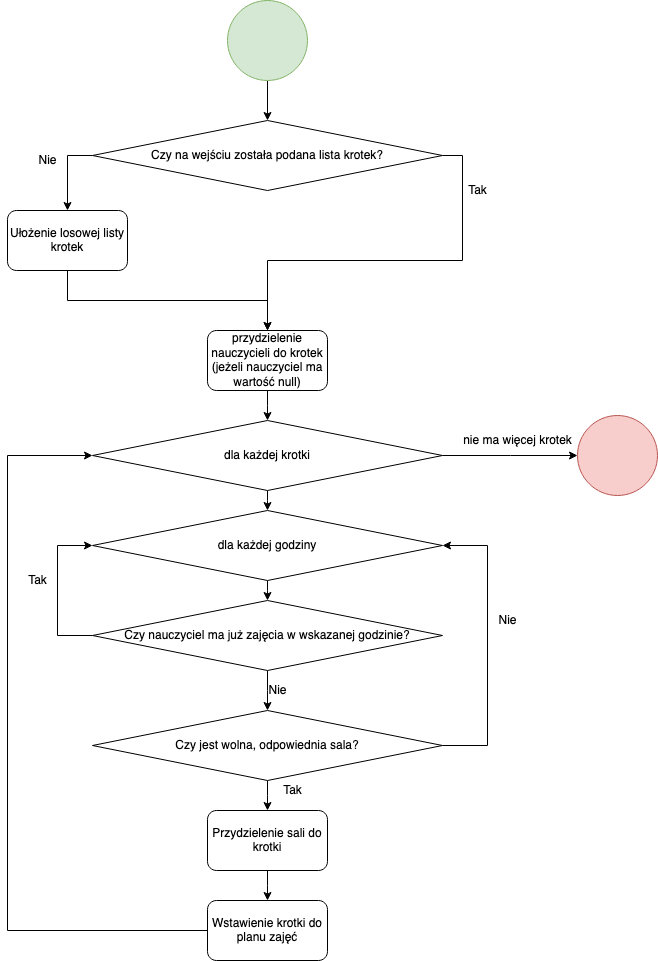
\includegraphics[width=\textwidth]{figures/time_table_prep}
\caption{Proces układania planu zajęć}\label{rys:time_table_prep}
\end{figure}

\begin{figure}[!ht]
\centering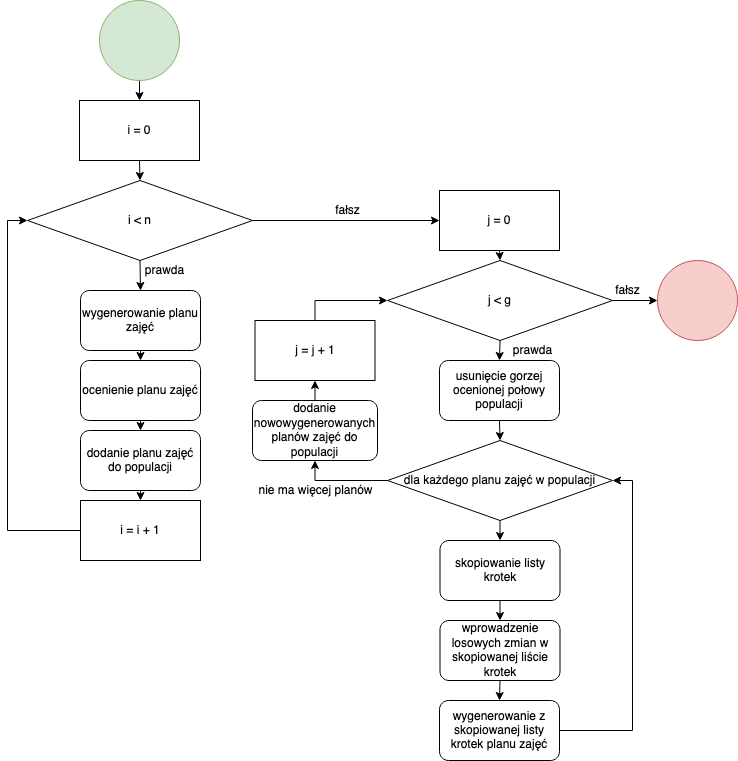
\includegraphics[width=\textwidth]{figures/alg_flow}
\caption{Algorytm -- diagram}\label{rys:alf_flow}
\end{figure}

\section{Funkcja oceny}

    Funkcja oceny przyznaje planowi zajęć pewną liczbę punktów. Ocena może mieć wartość z zakresu od minus nieskończoności do 0, gdzie im wartość większa, tym lepsza ocena.
    Wpływ na końcową ocenę mają następujące elementy:
\begin{enumerate}
	\item liczba tzw. okienek występujących w planie zajęć każdego nauczyciela,
	\item liczba tzw. okienek występujących w planie zajęć każdej klasy,
	\item liczba trudnych przedmiotów w ciągu jednego dnia w planie zajęć każdej klasy,
	\item liczba sytuacji, w których klasa ma rozdzielone zajęcia tego samego przedmiotu innym przedmiotem (np. 1. godzina lekcyjna -- matematyka, 2. godzina lekcyjna -- biologia, 3. godzina lekcyjna -- matematyka),
	\item liczba sytuacji, w których zajęcia wychowania fizycznego nie występują na początku lub na końcu planu zajęć dnia.
\end{enumerate}


\section{Ewolucja planów zajęć}

    Część ewolucyjna algorytmu wykorzystuje wszystkie poprzednie części. Na początku algorytm generuje pewną populację planów zajęć, która będzie nazywana dalej pierwszą generacją. Zawartość listy krotek jest identyczna dla każdej jednostki z populacji, ale kolejność krotek w liście jest pseudolosowo zmieniona. Dzięki takiemu rozwiązaniu, każda jednostka w populacji może wygenerować zupełnie inny plan zajęć. Za pomocą funkcji oceny, do każdego z planów zostaje przydzielona pewna liczba punktów. 

Połowa najgorzej ocenionych planów zostaje zabita. Z każdego planu zajęć, któremu udało się przeżyć, generowany jest kolejny plan. Plan, z którego został wygenerowany nowy plan, będzie nazywany w dalszej części pracy rodzicem, natomiast nowo wygenerowany plan będzie nazywany potomkiem. Lista krotek potomka, będzie zawierała tę samą kolejność co rodzic, ale losowo wybrane rekordy zamienią się w sposób pseudolosowy pozycjami w liście, taka zamiana będzie nazywana dalej mutacją. Nowo wygenerowane jednostki zostają ocenione oraz dodane do populacji, w ten sposób powstaje druga generacja planów zajęć.

    Czynność z poprzedniego akapitu powtarza się jeszcze g-razy, gdzie g to liczba wszystkich generacji. Działanie całego algorytmu zostało przedstawione na ~rysunku~\ref{rys:alf_flow}.


\section{Wielowątkowość}

Podczas implementacji algorytmu była rozważana oraz testowana możliwość zrównoleglenia części kodu. Mowa konkretnie pętli o iterującej się przez każdy plan w populacji, w celu wygenerowania nowego, zmutowanego. Nie spowodowało to jednak znaczącego przyśpieszenia działania algorytmu. Biorąc pod uwagę jeszcze fakt, że algorytm ostatecznie działa na maszynie jednowątkowej, pomysł implementacji rozwiązania wielowątkowego został porzucony.


\section{Parametry}
Algorytm przewiduje parametryzację trzech zmiennych:
\begin{itemize}
	\item rozmiar populacji \textit{p},
	\item liczbę wszystkich generacji utworzonych podczas działania algorytmu \textit{g},
	\item liczbę mutacji wprowadzonych do nowotworzonego planu zajęć \textit{m}.
\end{itemize}

Największy wpływ na końcową ocenę końcową ma parametr \textit{g}. Zakładając, że parametry \textit{p} i \textit{m} są stałe, to wartość parametru \textit{g} zależy liniowo od czasu wykonywania algorytmu oraz logarytmicznie od końcowej oceny. Im większy parametr \textit{g}, tym większa będzie końcowa ocena, ale im większa wartość \textit{g}, tym mniejszy jest wzrost oceny końcowej. Ostatecznie parametry zostały ustawione następująco:
\begin{itemize}
	\item \textit{p} = 10,
	\item \textit{g} = 1000,
	\item \textit{m} = 10.
\end{itemize}